\documentclass[a4paper]{article}
\usepackage{amsmath} % for multi-line aligned equations
\usepackage{enumitem} % for bullet points
\usepackage{graphicx} % for displaying images
\graphicspath{ {./Images/} } % search path for images
\usepackage{booktabs} % for making tables in professional style with top and bottom border
\usepackage{textcomp} % for degree symbol
\usepackage{fullpage} % for reducing page margins

%opening
\title{Libration Point Orbit Rendezvous Technique Using Linearized Relative Motion Dynamics and Nonlinear Differential Correction}
\author{Sara Case\\ Department of Aerospace Engineering\\ University of Maryland, College Park}
\date{Spring 2015}

\begin{document}

\maketitle


\section{Introduction}

The history of satellites being deployed to libration point orbits dates back to 1978, when ISEE-3 was launched to the Sun-Earth L1 point. ACE, WIND, SOHO are currently orbiting the same point, with the DSCOVR and LPF satellites set to join them in 2015.  Several spacecraft have been deployed to the Sun-Earth L2 point, and the ARTEMIS mission explored L1 and L2 in the Earth-Moon system.  Several additional libration point orbiting missions are currently planned, including the James Webb Space Telescope.  So far, all libration point missions have consisted of a single satellite which operates independently of any other satellite.  There is research on deploying a formation of satellites to fly together around libration points.  However, not much research has been performed regarding rendezvous with libration point orbiters.  %  TODO: (give examples of formation flying research)

Libration point orbit rendezvous would be a critical component for many possible mission architectures.  If a large satellite needs to be launched in components and assembled in orbit, the individual components would need to perform rendezvous and docking prior to assembly.  If a valuable space asset such as a telescope requires an on-orbit repair, the satellite servicing mission will need to rendezvous with the object.  A libration point orbit could be a useful place to build a space station, and in that case rendezvous capabilities would be important during the construction of the station as well as every crew and cargo mission to visit the station. % TODO: (refer to a paper about building a space station at a libration point)

Satellite rendezvous in low-Earth orbit is well-studied, due to many years of experience operating the International Space Station and other applications.  The Hill's / Clohessy-Wiltshire equations can be used to estimate the relative motion of a chaser vehicle with respect to a target vehicle in a circular orbit.  These equations of relative motion can be used to compute the estimated \(\Delta V\) (instantaneous change in velocity) to travel between waypoints defining an approach trajectory.  However, for libration point orbits, the dynamical environment is quite different and the same equations of motion can not be used. % TODO: (cite rendezvous ISS paper) (mention r-bar, v-bar?)

Luquette \cite{luquette2004} has developed linearized equations of relative motion for formation flying in libration point orbits.  Lian et al. \cite{lian2011} have used these linearized dynamics to compute impulses for a chaser satellite to travel between waypoints in order to approach a target orbiting a libration point.  This paper discusses the results of this technique, and presents an additional step in which the shooting method is used to refine the computed \(\Delta V\) for use in nonlinear propagation.

\section{Dynamics}

\subsection{Circular Restricted Three-Body Dynamics}
The circular restricted three body problem (CRTBP) deals with two larger objects orbiting each other and a third object of infinitesimal mass.  Examples include a man-made satellite orbiting in the Sun-Jupiter system, or the Earth-Moon system.  When dealing with the Sun-Earth system, the second body is often modeled by treating the Earth and Moon as a single object at the Earth-Moon barycenter; this is called the Sun-Earth/Moon system.

The nonlinear equations of motion for a satellite in the CRTBP are:

\begin{equation} \label{eq:CRTBP}
\begin{aligned}
\ddot{x} &= x + 2\dot{y} + \frac{(1 - \mu)(-\mu - x)}{r_1^3} + \frac{\mu(1 - \mu - x)}{r_2^3} \\
\ddot{y} &= y - 2\dot{x} - \frac{(1 - \mu)y}{r_1^3} - \frac{\mu y}{r_2^3} \\
\ddot{z} &= \frac{-(1 - \mu)z}{r_1^3} - \frac{\mu z}{r_2^3}
\end{aligned}
\end{equation}

where \(r_1\) and \(r_2\) are the distances from the larger and smaller bodies to the target satellite:

\begin{equation*}
\begin{aligned}
r_1 &= \sqrt{(x-\mathbf{X_1}(0))^2 + y^2 + z^2} \\
r_2 &= \sqrt{(x-\mathbf{X_2}(0))^2 + y^2 + z^2}
\end{aligned}
\end{equation*}

and \(\mathbf{X_1}\) and \(\mathbf{X_2}\) are the positions of the larger and smaller bodies along the rotating RTBP frame X-axis:

\begin{equation*}
\begin{aligned}
\mathbf{X_1} &= \begin{bmatrix}
						-\mu \\ 0 \\ 0 
						\end{bmatrix} \\
\mathbf{X_2} &= \begin{bmatrix}
						1 - \mu \\ 0 \\ 0
						\end{bmatrix}
\end{aligned}
\end{equation*}

(Need to provide definition of \(\mu\))

\subsection{Linearized CRTBP Relative Motion Dynamics}
Luquette \cite{luquette2004} has derived linearized equations of relative motion of a chaser satellite with respect to a target satellite orbiting in the restricted three body problem (RTBP).  He provides the equations of motion in two reference frames: the inertial frame as well as the rotating (RTBP) frame.  These equations of motion are valid anywhere in the RTBP system; they are not assumed to be near any specific libration point.

The equations of relative motion of a chaser satellite with respect to a target satellite, given in the RTBP reference frame, are:

(not including SRP; assuming no thrust)

(should I also include the inertial version of the relmo EOM's from Luquette?  I only used the rotating frame version, but maybe the inertial version should also be provided for completeness.  Could simply say that the inertial version doesn't have the \(\omega\) terms and all the vectors are in the inertial frame instead of CRTBP.)

\begin{equation} \label{eq:RelmoDerivs}
\dot{\boldsymbol{\xi}}_R = \mathbf{A}_R(t)\boldsymbol{\xi}_R
\end{equation}

where \(\boldsymbol{\xi}_R\) is the state/offset of the chaser vehicle with respect to the target vehicle in the rotating frame (come up with different symbols to use than x and xdot because already used x above):

\begin{equation*}
\boldsymbol{\xi}_R = \begin{bmatrix}
									\mathbf{x}_R \\
									\dot{\mathbf{x}}_R
									\end{bmatrix}
\end{equation*}

\(\mathbf{A}_R(t)\) is the 6\(\times\)6 linearized relative motion dynamics matrix in the rotating frame: (note in the paper I'm citing, he says \(-2 [\boldsymbol{\omega} \times]^T\), but in his PhD it just says \(-2 [\boldsymbol{\omega} \times]\) which seems to be correct)

\begin{equation} \label{eq:RelmoDynMatrix}
\mathbf{A}_R(t) = \begin{bmatrix}
								\mathbf{0}          & \mathbf{I_3} \\
								\mathbf{\Xi}_R(t) & -2 [\boldsymbol{\omega} \times]
								\end{bmatrix}
\end{equation}

where

\begin{equation*}
\mathbf{\Xi}_R(t) = -(c_1 + c_2)\mathbf{I_3} 
								+ 3c_1\mathbf{\hat{r}_1}(t) \mathbf{\hat{r}_1}(t)^T 
								+ 3c_2\mathbf{\hat{r}_2}(t) \mathbf{\hat{r}_2}(t)^T 
								+ [\boldsymbol{\dot{\omega}} \times] 
								- [\boldsymbol{\omega}\times][\boldsymbol{\omega}\times]
\end{equation*}

and

\begin{equation*}
\begin{aligned}
c_1 &= \frac{1- \mu}{r_1^3} \\
c_2 &= \frac{\mu}{r_2^3}
\end{aligned}
\end{equation*}

Note that \(\boldsymbol{\omega}\) is the rotation rate of the rotating RTBP frame with respect to the inertial frame:
\begin{equation*}
\boldsymbol{\omega} = \begin{bmatrix}
					0 \\ 
					0 \\
					\omega
					\end{bmatrix}
\end{equation*}

And  \([\boldsymbol{\omega}\times]\) is the cross-product matrix of \(\boldsymbol{\omega}\), so we get:
\begin{equation*}
[\boldsymbol{\omega}\times] = \begin{bmatrix}
								0           & -\omega & 0 \\ 
								\omega & 0             & 0 \\
								0           & 0             & 0
								\end{bmatrix}
\end{equation*}

Also note that if we assume that the rotation rate is constant (that is, assume we can use the CRTBP where the massive bodies are in circular orbits around each other), then the \(\boldsymbol{\dot{\omega}}\) term cancels to zero.

(Another note to possibly mention: \\ In non-dimensional units, \(\omega = \sqrt{GM/r^3} = 1\).)

In order to integrate a chaser satellite's trajectory using the equations of relative motion given in Equation \ref{eq:RelmoDerivs}, the integration state vector must contain the absolute state of the target satellite in the CRTBP frame (with respect to the origin of the CRTBP frame) and the relative state of the chaser satellite in the CRTBP frame (with the origin located at the target satellite).  The target satellite's state over time can be integrated using the classical CRTBP equations of motion as given in Equation \ref{eq:CRTBP}, which must be done concurrently with the integration of the relative motion of the chaser so that the time-dependent linearized relative motion dynamics matrix \(\mathbf{A}_R(t)\) given in Equation \ref{eq:RelmoDynMatrix} can be computed.

\section{Traveling Between Waypoints with Impulsive \(\Delta V\)'s}

(Introduce the idea of waypoints here - divide the approach into a series of shorter arcs defined wrt the target.  Probably this is where we should provide background info on Hills/CW.)

\subsection{Using the Linearized Relative Motion Dynamics Matrix to Compute \(\Delta V\)}

The linearized relative motion dynamics matrix given in Equation \ref{eq:RelmoDynMatrix} can also be used to numerically accumulate a State Transition Matrix (STM), \(\boldsymbol{\Phi}\), of the chaser satellite with respect to the target satellite over time:

\begin{equation} \label{eq:STM}
\dot{\boldsymbol{\Phi}} = \mathbf{A}_R(t)\boldsymbol{\Phi}
\end{equation}

The initial ``state vector" for the STM passed to the integration process should be the \(6\times6\) identity matrix, \(\mathbf{I_6}\).  As above, the STM must be integrated concurrently with the target satellite's state because of the time-dependence in \(\mathbf{A}_R(t)\).  When integrated from the initial state at time \(t_i\) to a future time \(t_{i+1}\), this accumulated State Transition Matrix represents the relative position and velocity of the chaser at time \(t_{i+1}\) with respect to its relative position and velocity at time \(t_i\).  More explicitly:

(need to make notation consistent; should it be r, v or x, xdot, or xi, xidot, or what)

\begin{equation}
\begin{bmatrix}
		\mathbf{r}_{i+1} \\
		\mathbf{v}_{i+1}
		\end{bmatrix}
= 
\begin{bmatrix}
		\boldsymbol{\Phi}_{11} & \boldsymbol{\Phi}_{12} \\
		\boldsymbol{\Phi}_{21} & \boldsymbol{\Phi}_{22}
		\end{bmatrix}
\begin{bmatrix}
		\mathbf{r}_i \\
		\mathbf{v}_i
		\end{bmatrix}
\end{equation}

This can be used to compute the required velocity \(\mathbf{v}_i^+\) for the chaser satellite to travel from waypoint \(\mathbf{r}_i\) to waypoint \(\mathbf{r}_{i+1}\) in time (\(t_{i+1} - t_i\)).  (Like you do with Hills/CW.)  Lian et. al. used this approach in paper 1 and paper 2.  Lian et. al. used the equations with J2000 reference axes and equations of motion written in J2000, rather than the rotating frame (RTBP) version being used here.

\begin{equation} \label{eq:RequiredVelocity}
\mathbf{v}_i^+ = \boldsymbol{\Phi}_{12}^{-1}(\mathbf{r}_{i+1} - \boldsymbol{\Phi}_{11}\mathbf{r}_i)
\end{equation}

The instantaneous change in velocity (\(\Delta V\)) for this maneuver is then simply the difference between the required velocity and the velocity that the chaser satellite had before the maneuver:

\begin{equation} \label{eq:DeltaV}
\Delta \mathbf{v}_i = \mathbf{v}_i^+ - \mathbf{v}_i^-
\end{equation}

\subsection{Shooting Method with Nonlinear Dynamics}

The approach described above for computing \(\Delta V\) is based on the linearized equations of relative motion developed by Luquette.  Of course, the true dynamical environment in the CRTBP is nonlinear, as seen in Equation \ref{eq:CRTBP}.

The linear-based estimate of \(\Delta V\) can be ``corrected" for the nonlinear propagation model using the shooting method.  The linear-based estimated velocity is used as an initial guess for the iterative differential correction process.  Each of the three components of the velocity vector is varied in order to achieve convergence on the desired three-dimensional waypoint \(\mathbf{w}_{desired}\) within some specified tolerance.

\begin{enumerate}[leftmargin=!,labelindent=12pt,itemindent=0pt, label=Step \arabic*:]

	\item Using the initial guess for the chaser relative velocity \(\mathbf{v}_i^+\), propagate both the target and chaser satellite from time \(t_i\) to \(t_{i+1}\) using the nonlinear CRTBP equations of motion and compute the nominally achieved waypoint \(\mathbf{w}_{i+1}\).
	
	\item Add to the x-component of the velocity a pre-chosen scalar value, called the perturbation.  Propagate the satellites from time \(t_i\) to \(t_{i+1}\) using this perturbed velocity and compute the achieved waypoint \(\mathbf{w}_{i+1}'\).
	
	\item Compute the difference between \(\mathbf{w}_{i+1}\) and \(\mathbf{w}_{i+1}'\), \(\frac{d\mathbf{w}}{dv_x}\).
	
	\item Reset the x-component of the velocity to its original value, and repeat steps 2 and 3 for the y-component of the velocity.
	
	\item Reset the y-component of the velocity to its original value, and repeat steps 2 and 3 for the z-component of the velocity.
	
	\item Gather the results into a partial derivatives matrix, \(\mathbf{M}\):
	
	\begin{equation} \label{eq:ShootingMethodPartialDerivs}
	\mathbf{M} = \left[ \frac{d\mathbf{w}}{d\mathbf{v}} \right]
	= \begin{bmatrix}
	\frac{dw_x}{dv_x} & \frac{dw_y}{dv_x} & \frac{dw_z}{dv_x} \\[0.3em]
	\frac{dw_x}{dv_y} & \frac{dw_y}{dv_y} & \frac{dw_z}{dv_y} \\[0.3em]
	\frac{dw_x}{dv_z} & \frac{dw_y}{dv_z} & \frac{dw_z}{dv_z}
	\end{bmatrix}
	\end{equation}
	
	\item Compute an updated guess for the velocity:
	
	\begin{equation} \label{eq:ShootingMethodUpdate}
	\mathbf{v}_i^+ = \mathbf{v}_i^+ + [\mathbf{M}]^{-1}(\mathbf{w}_{desired} - \mathbf{w}_{i+1 achieved})
	\end{equation}
	
\end{enumerate}

Repeat steps 1 through 7 until all three components of \(\mathbf{w}_{achieved}\) converge to \(\mathbf{w}_{desired}\) within some tolerance.

(Need to go through all section 2 and section 3 equations/symbols and make symbol usage consistent.)

\subsection{Definition of Waypoint Reference Frames}

In this work, two local reference frames are defined with respect to the target satellite's orbit around its libration point.  Each of these frames will rotate once for each full orbit of the target around the libration point.

The two libration points of most interest for this work are \(L_1\) and \(L_2\).  The position of \(L_1\) in the CRTBP frame is found by computing the real root \(l_1\) of this polynomial in \(x\):

\begin{equation} \label{eq:L1}
(1 - \mu)(p^3)(p^2 - 3p + 3) - \mu(p^2 + p + 1)(1 - p)^3 = 0
\end{equation}

where:

\begin{equation*}
p = 1 - \mu - x
\end{equation*}

The coordinates of \(L_1\) are then \([l_1, 0, 0]\) in the CRTBP frame.  Likewise, the position of \(L_2\) in the CRTBP frame is found by computing the real root \(l_2\) of this polynomial in \(x\):

\begin{equation} \label{eq:L2}
(1 - \mu)(p^3)(p^2 + 3p + 3) - \mu(p^2 + p + 1)(1 - p)(p + 1)^2 = 0
\end{equation}

where:

\begin{equation*}
p = \mu - 1 + x
\end{equation*}

The coordinates of \(L_2\) are then \([l_2, 0, 0]\) in the CRTBP frame.

Local RIC and VNB reference frames are then defined with the origin of both of these frames located at the target satellite's position.  The RIC, or ``radial-intrack-crosstrack," frame as has its first primary axis the vector pointing from the libration point radially out to the target satellite.  For example, in the case of a target satellite orbiting \(L_1\), the fundamental \(\mathbf{\hat{R}}\), \(\mathbf{\hat{I}}\), and \(\mathbf{\hat{C}}\) axes of the RIC frame are defined as:

\begin{equation} \label{eq:RIC}
\begin{aligned}
\mathbf{\hat{R}} &= \widehat{\mathbf{x} - \mathbf{L}_1} \\
\mathbf{\hat{C}} &= \widehat{\mathbf{R} \times \mathbf{\dot{x}}} \\
\mathbf{\hat{I}} \, &= \widehat{\mathbf{C} \times \mathbf{R}}
\end{aligned}
\end{equation}

where \(\mathbf{x}\) and \(\mathbf{\dot{x}}\) are the target satellite's position and velocity vectors in the CRTBP frame.

The VNB, or ``velocity-normal-binormal," frame has as its first primary axis the target satellite's velocity vector.  In the case of a target satellite orbiting \(L_1\), the fundamental \(\mathbf{\hat{V}}\), \(\mathbf{\hat{N}}\), and \(\mathbf{\hat{B}}\) axes of the VNB frame are defined as:

\begin{equation} \label{eq:VNB}
\begin{aligned}
\mathbf{\hat{V}} &= \mathbf{\dot{\hat{x}}} \\
\mathbf{\hat{N}} &= \widehat{\mathbf{R} \times \mathbf{V}}  \\
\mathbf{\hat{B}} &= \widehat{\mathbf{V} \times \mathbf{N}} 
\end{aligned}
\end{equation}

\section{Results}

\subsection{Performance of Linear \(\Delta V\) Estimate and Shooting Method}

To begin evaluating the performance of the techniques presented above, consider the following scenario.  The target satellite is in a planar Lyapunov orbit around the Earth-Moon L1 point as shown in Figure \ref{fig:FullOrbit_1}.  The target satellite's initial conditions are presented in Table \ref{tab:IC_1}.  For this test, the rendezvous starts with the target satellite on the CRTBP +X-axis, that is, crossing the XZ-plane.

\begin{table}[h] \label{tab:IC_1}
	\begin{center}
		\begin{tabular}{l l}
			\toprule
			Parameter   & Value \\
			\midrule
			X                & 0.862307159058101 \\
			Z                & 0.0 \\
			\(\dot{Y}\) & -0.187079489569182 \\
			Period        & 2.79101343456226 \\
			\bottomrule
		\end{tabular}
		\caption{Initial Conditions of the Target Satellite in the CRTBP Frame}
	\end{center}
\end{table}

\begin{figure}[h] \label{fig:FullOrbit_1}
	\begin{center}
		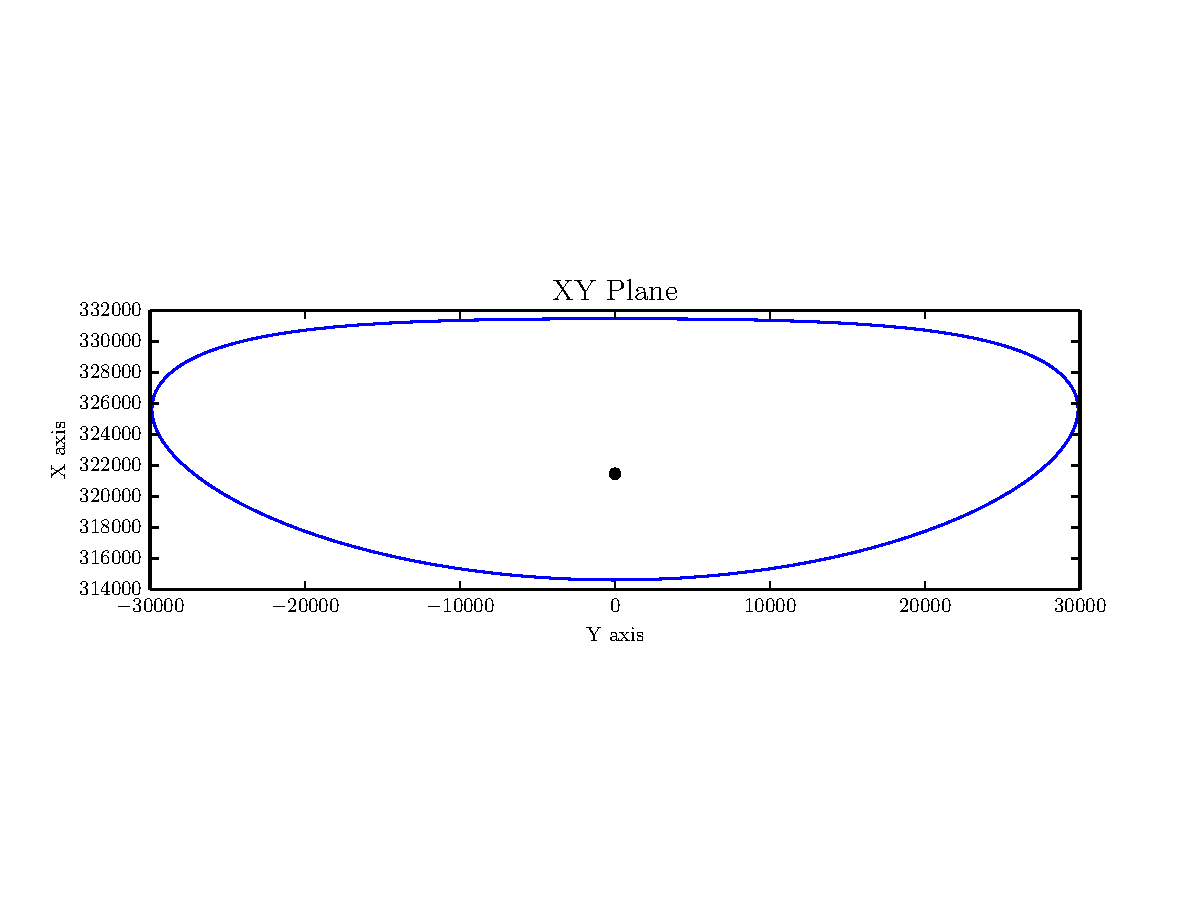
\includegraphics[width=0.9\textwidth]{Target_Full_Orbit_1}
		\caption{Target Satellite Orbit in Earth-Moon L1 CRTBP Frame}
	\end{center}
\end{figure}

The initial conditions in Table \ref{tab:IC_1} are provided in non-dimensional units.  To convert between non-dimensional and dimensional units, the relevant properties of the Earth-Moon CRTBP system are presented in Table \ref{tab:Environment_1}.

\begin{table}[h] \label{tab:Environment_1}
	\begin{center}
		\begin{tabular}{l l}
			\toprule
			Parameter   & Value \\
			\midrule
			Earth mass (kg) & 5.97219e24 \\
			Moon mass (kg) & 7.34767309e22 \\
			Mass ratio \(\mu\)      & 0.012277471 \\
			Combined mass (kg), or 1 MU & 6.045667e+24 \\
			\(r_{12}\) (km), or 1 DU & 384400.0 \\
			Time Constant (s), or 1 TU & 375201.9 \\
			Period of Moon around Earth (s) & 2\(\pi\)TU \\
			\bottomrule
		\end{tabular}
		\caption{Earth-Moon CRTBP Parameters}
	\end{center}
\end{table}

Three waypoints are defined for the chaser satellite to travel along on its rendezvous with the target, with a final ``waypoint'' located at the target satellite itself.  The waypoints are presented in Table \ref{tab:Waypoints_1} in the RIC reference frame.  The waypoints are converted into the CRTBP frame for the propagation.  Note that these waypoints represent an approach along the \(\mathbf{I}\) axis of the RIC frame.  

\begin{table}[h] \label{tab:Waypoints_1}
	\begin{center}
		\begin{tabular}{ccccc}
			\toprule
			Waypoint   & Time (days) & R (km) & I (km) & C (km) \\
			\midrule
			1 & 0.00 & 0.0 & 15.0 & 0.0 \\
			2 & 0.36 & 0.0 & 5.0 & 0.0 \\
			3 & 0.97 & 0.0 & 1.0 & 0.0 \\
			4 & 1.59 & 0.0 & 0.0 & 0.0 \\
			\bottomrule
		\end{tabular}
		\caption{Waypoints in RIC Frame}
	\end{center}
\end{table}

Figure \ref{fig:RIC_1} shows the result of propagating the target and chaser satellite through a rendezvous using these waypoints.  The integration is done in the CRTBP frame, and the results are converted to the RIC frame for the plot, with the target spacecraft at the origin and the chaser spacecraft offset with respect to the target shown in kilometers.  The green curve shows the path of the chaser satellite when propagated using the linear relative motion dynamics as given in Equation \ref{eq:RelmoDerivs}, with the application of impulsive \(\Delta V\)'s as computed using Equation \ref{eq:RequiredVelocity}.  The red curve shows the result when the chaser satellite is propagated using the nonlinear CRTBP dynamics as shown in Equation \ref{eq:CRTBP}; the nominal \(\Delta V\)'s as computed using the linear model are still applied.  It is easily seen that the nominally planned maneuvers do not bring the chaser precisely to the desired waypoints when propagating with the nonlinear model.  Finally, the blue curve shows the result when the chaser satellite is propagated using the nonlinear CRTBP dynamics when the \(\Delta V\)'s have been corrected through the iterative shooting method process as shown in Equation \ref{eq:ShootingMethodUpdate}.  The path does not precisely match the original green curve due to the different dynamical models in use; however, each waypoint is achieved successfully.  (Also note that the image axes are not scaled equally.)

\begin{figure}[h] \label{fig:RIC_1}
	\begin{center}
		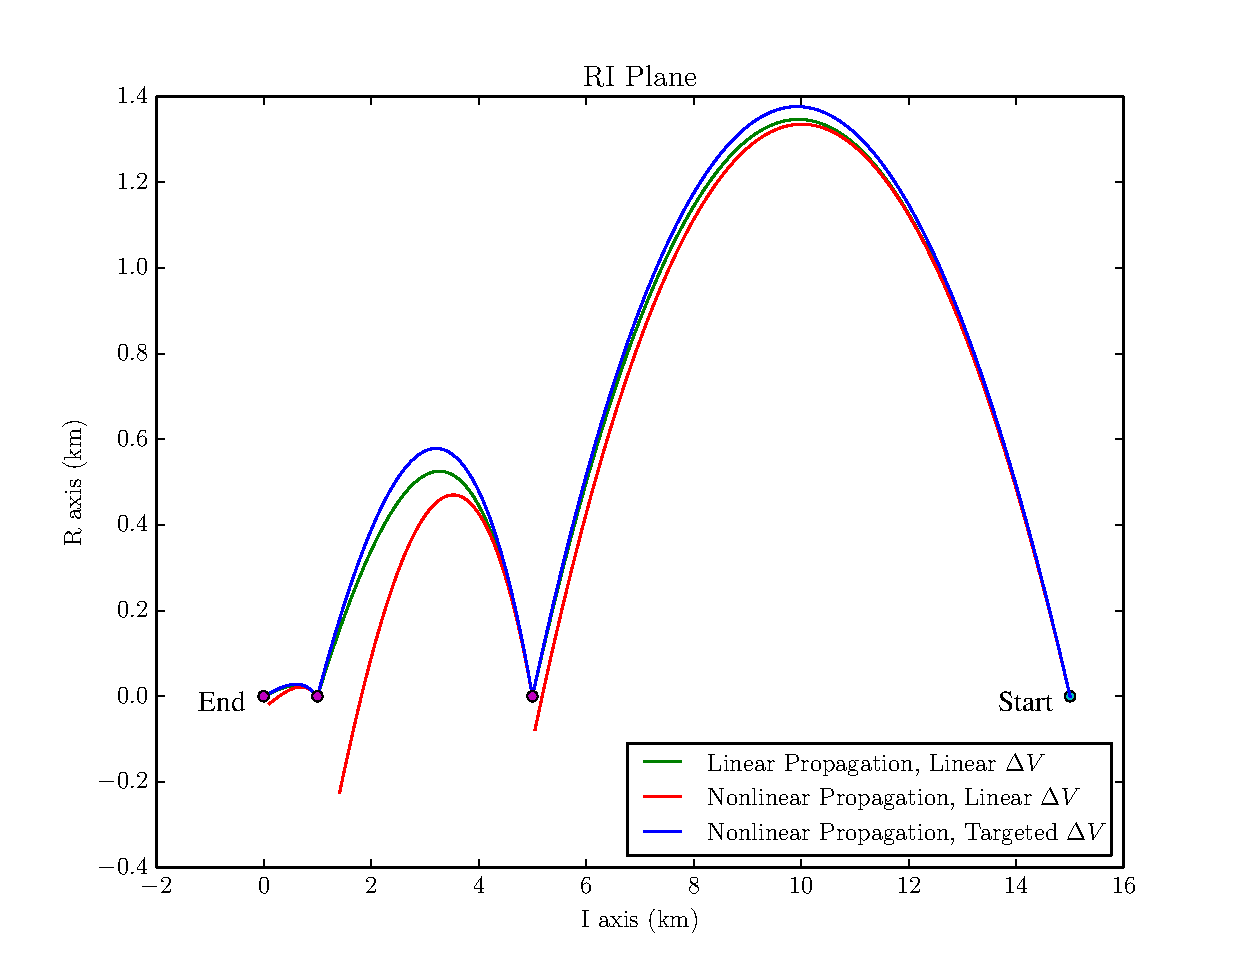
\includegraphics[width=0.9\textwidth]{RIC_1}
		\caption{Relative Motion of a Chaser Satellite with respect to a Target}
	\end{center}
\end{figure}

The results for this case are also summarized in Table \ref{tab:Results_1}.  To compute the \(\Delta V\) values, the chaser satellite was assumed to start precisely from waypoint 1 with its pre-maneuver velocity at waypoint 1 equal to the target satellite's initial velocity in the CRTBP frame.  The final maneuver at waypoint 4 is computed to make the chaser's velocity equal to the target satellite's velocity to complete the rendezvous.

We can note that, while the difference in \(\Delta V\) magnitude is quite small between the linear computation and the targeted computation, on the order of millimeters/second, the angular difference between the two \(\Delta V\) vectors reaches almost 6\textdegree at waypoint 3.  These differences result in achieved position errors on the order of hundreds of meters at each waypoint when the linear estimate is applied in the nonlinear frame; the errors are reduced to the order of centimeters when the shooting method is applied.

For the tuning parameters of the shooting method, the perturbation value for the velocity components was set to 1e-5 DU/TU (or SU for speed units) or about 1.0 centimeters/second.  The tolerance on the achieved waypoints was set to 1e-9 DU or about 0.38 meters.  The maximum number of allowed iterations was set to 10; if the desired tolerance is not achieved within 10 iterations, the process will continue with the value achieved by the \(10^{th}\) iteration.

\begin{table}[h] \label{tab:Results_1}
	\begin{center}
		\begin{tabular}{c p{1cm} p{1cm} p{1.5cm} p{1.5cm} p{1.5cm} p{1.5cm}}
			\toprule
			Waypoint   & Linear \(\Delta V\) (m/s) & Targeted \(\Delta V\) (m/s) & \(\Delta V\) Angle Difference (deg) & \(\Delta V\) Magnitude Difference (m/s) & Linear Position Error (m) & Targeted Position Error (m) \\
			\midrule
			1 & 0.346 &	0.345 &	0.466 &	-0.001 &	N/A &	N/A \\
			2 & 0.293 &	0.295 &	2.609 &	0.002 &	91.394 &	0.011 \\
			3 & 0.064 &	0.059 &	5.890 &	-0.005 &	470.653 &	0.063 \\
			4 & 0.019 &	0.018 &	0.445 &	-0.001 &	107.663 &	0.056 \\
			Total & XX  & XX &  & XX &  & \\
			\bottomrule
		\end{tabular}
		\caption{\(\Delta V\) and Position Error at each Waypoint}
	\end{center}
\end{table}

(Note that we use the *new* achieved waypoint to re-compute the linear dV estimate for the next waypoint before then targeting the next waypoint)

\subsection{Rendezvous Approach Directions}

This technique can be used to evaluate the relative \(\Delta V\) cost of performing a rendezvous at different points along the target spacecraft's orbit.  The following results present twelve test cases that each begin with the target satellite at a different ``clock angle" in its orbit; each test case begins 30\textdegree apart, as indicated by the asterisks shown in Figure \ref{fig:FullOrbit_2}.

\begin{figure}[h] \label{fig:FullOrbit_2}
	\begin{center}
		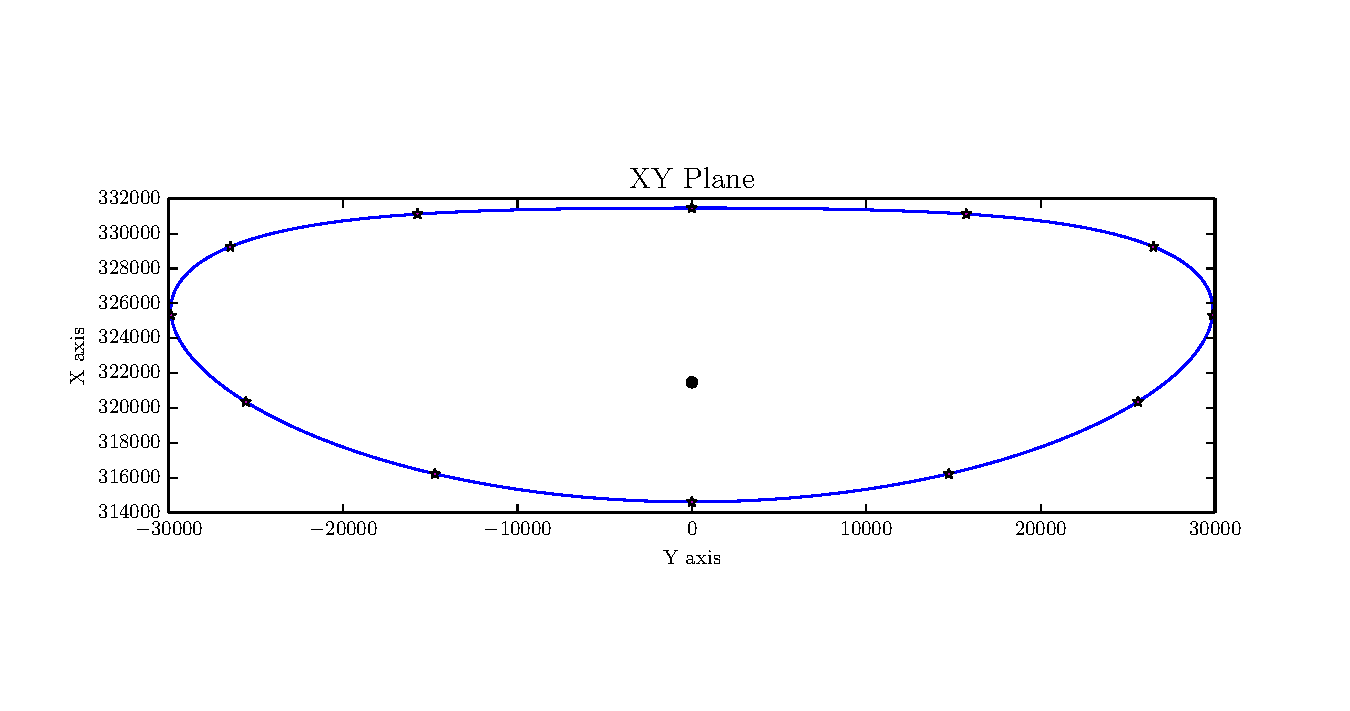
\includegraphics[width=0.9\textwidth]{Target_Full_Orbit_2}
		\caption{Twelve Target Satellite Initial Conditions with 30\textdegree Clock Angle Spacing}
	\end{center}
\end{figure}

Each of these twelve rendezvous sequences are computed using the waypoint locations defined in the RIC frame as shown in Table \ref{tab:Waypoints_1}.  However, due to the different local curvature of the target orbit at each of the twelve starting locations, the relative motion patterns in the RIC frame for each rendezvous are different, as shown in Figure \ref{fig:RIC_2}.  When viewed using the CRTBP rotating libration point frame as in Figure \ref{fig:RLP_2}, it is more intuitively seen that each rendezvous approaches the target satellite from a different direction in the CRTBP frame, due to the rotation of the RIC frame with the target satellite's orbit.

\begin{figure}[h] \label{fig:RIC_2}
	\begin{center}
		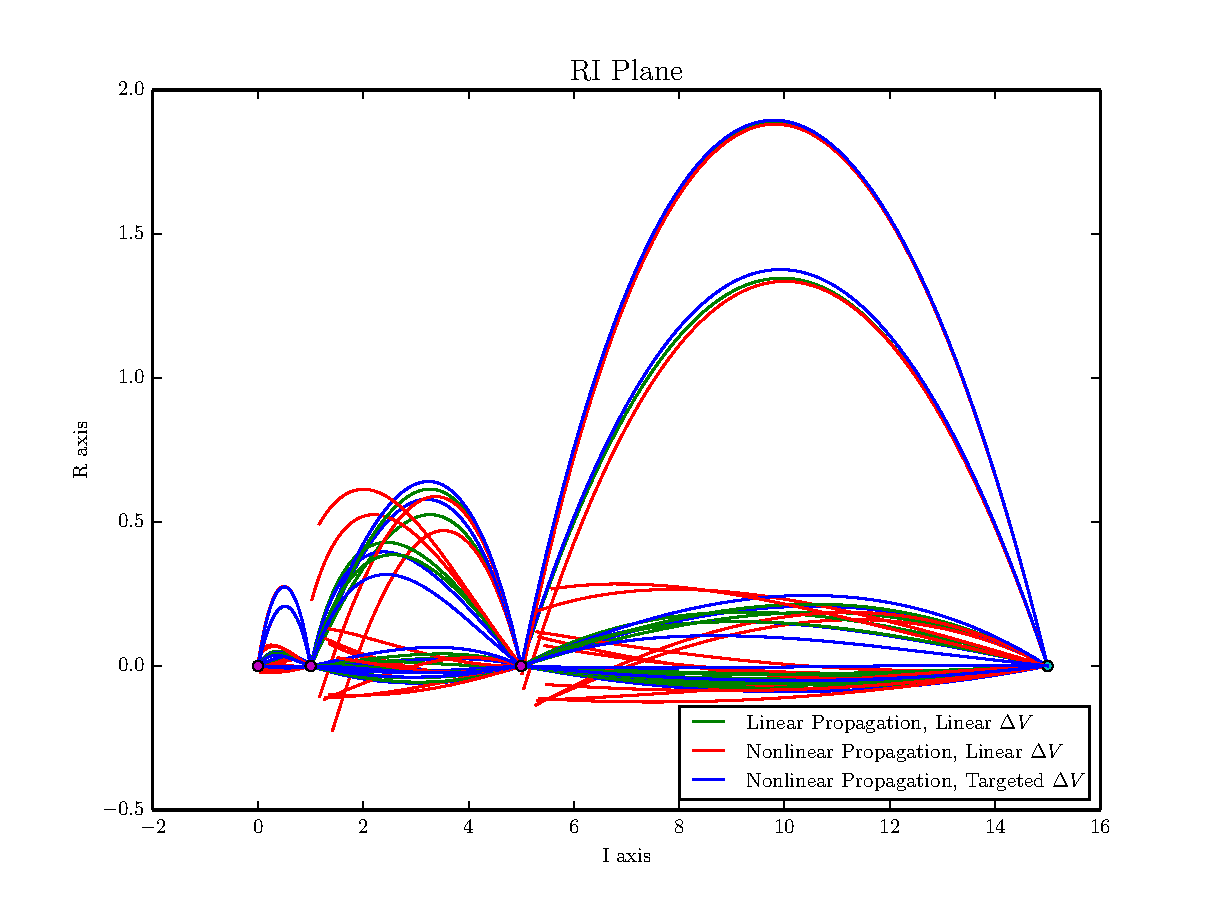
\includegraphics[width=0.9\textwidth]{RIC_2}
		\caption{Relative Motion of Chaser Satellite with respect to a Target using Initial Conditions with 30\textdegree Clock Angle Spacing; RIC Frame}
	\end{center}
\end{figure}

\begin{figure}[h] \label{fig:RLP_2}
	\begin{center}
		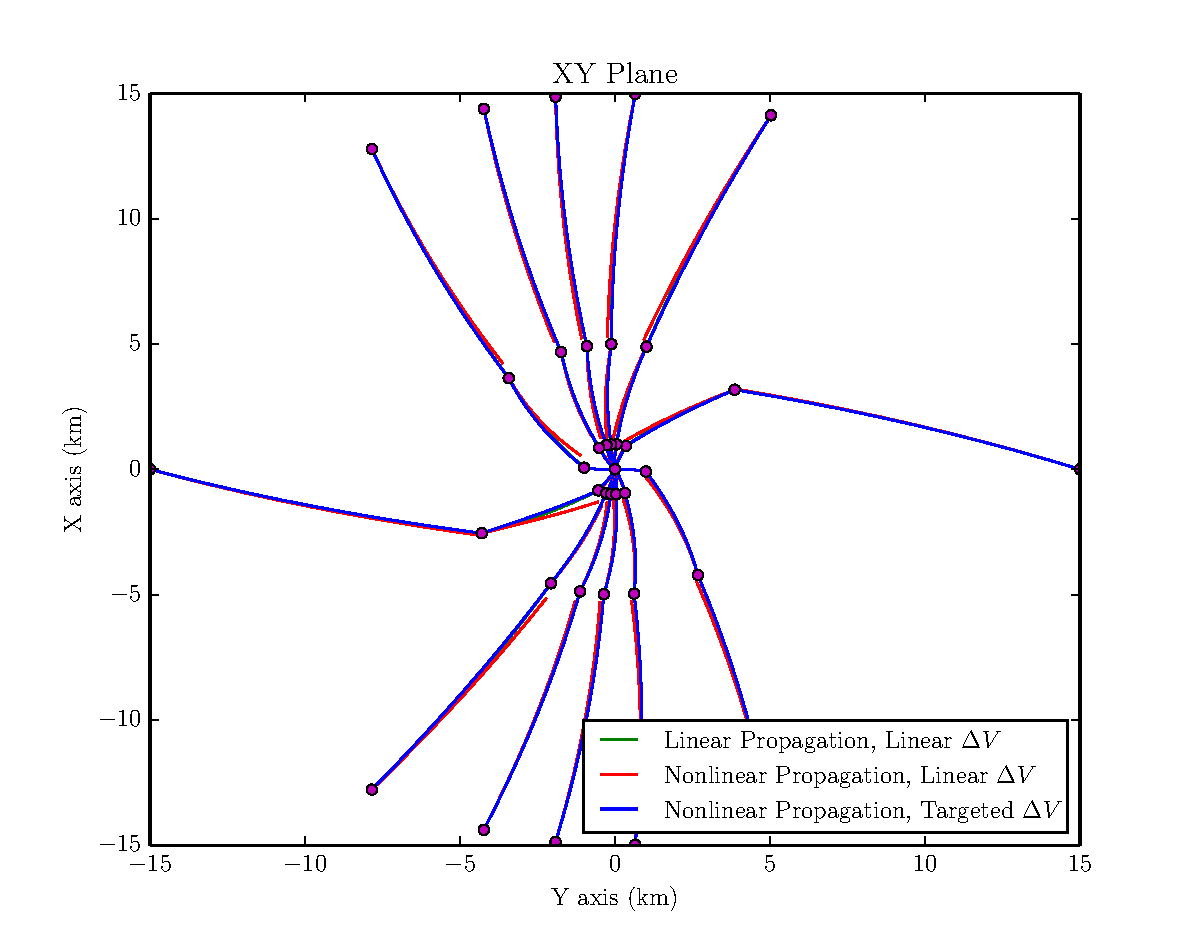
\includegraphics[width=0.9\textwidth]{RLP_2}
		\caption{Relative Motion of Chaser Satellite with respect to a Target using Initial Conditions with 30\textdegree Clock Angle Spacing; CRTBP Frame}
	\end{center}
\end{figure}

\section{Notes to Self}

Show cases where we approach from different directions (+/-R, +/-I, +/-C)

Evaluate relative cost of approaching in different ways

Distance (maybe percentage of orbit covered?) where this technique doesn't work

Seems like shorter times maybe gives better behavior of the linear dV estimate?  Longer time = more need to use the targeter?

Show what happens if you miss a maneuver

Kinda interesting to show in RLP, VNB

Maybe talk about measuring the "excursion" of the trajectory (perpendicular to the vector from one waypoint to the next)

\section{Conclusions}

Technique can be used for any LPO (Lyapunov, halo, Lissajous) for any RLP system or L-point

\bibliographystyle{unsrt}
\bibliography{LPORendezvous}

\end{document}
